%\documentclass[twocolumn,showpacs,aps,superscriptaddress,eqsecnum,prd,notitlepage,showkeys,fleqn,usenatbib,useAMS]{revtex4-1}
\documentclass[RNAAS,twocolumn]{aastex63}

\usepackage{amssymb}
\usepackage{amsmath}
\usepackage{graphicx}
\usepackage{dcolumn}
\usepackage{hyperref}
\usepackage{color,units}
\usepackage{aas_macros}
\usepackage{lineno}
\usepackage{xspace}
\usepackage{subfigure}
\usepackage{comment}
\usepackage{newtxtext,newtxmath}

\usepackage[normalem]{ulem} %% for striking out text





%% affiliation shortcuts
\newcommand{\BHI}{Black Hole Initiative, Harvard University, Cambridge, MA 02138, USA}
\newcommand{\CFA}{Center for Astrophysics $\vert$ Harvard \& Smithsonian, Cambridge, MA 02138, USA}


\begin{document}


\title{
Local Abundance of Ultra-Massive Black Holes.
}

% Add ORCIDs
\author[0000-0002-4831-2105]{Nadav Joseph Outmezguine}
    \email{Nadav.Out@gmail.com}
\affiliation{Raymond and Beverly Sackler School of Physics and Astronomy, Tel-Aviv University, Tel-Aviv 69978, Israel}
\affiliation{Berkeley Center for Theoretical Physics, Department of Physics, University of California, Berkeley, CA 94720, U.S.A.}
\affiliation{Theoretical Physics Group, Lawrence Berkeley National Laboratory, Berkeley, CA 94720, U.S.A}

\author[0000-0001-9879-7780]{Fabio Pacucci}
\affiliation{\CFA}
\affiliation{\BHI}

\author[0000-0003-4330-287X]{Abraham Loeb}
\affiliation{\CFA}
\affiliation{\BHI}


\begin{abstract}
Local statistics of huge black holes etc.
\end{abstract}

\section{Introduction}

% 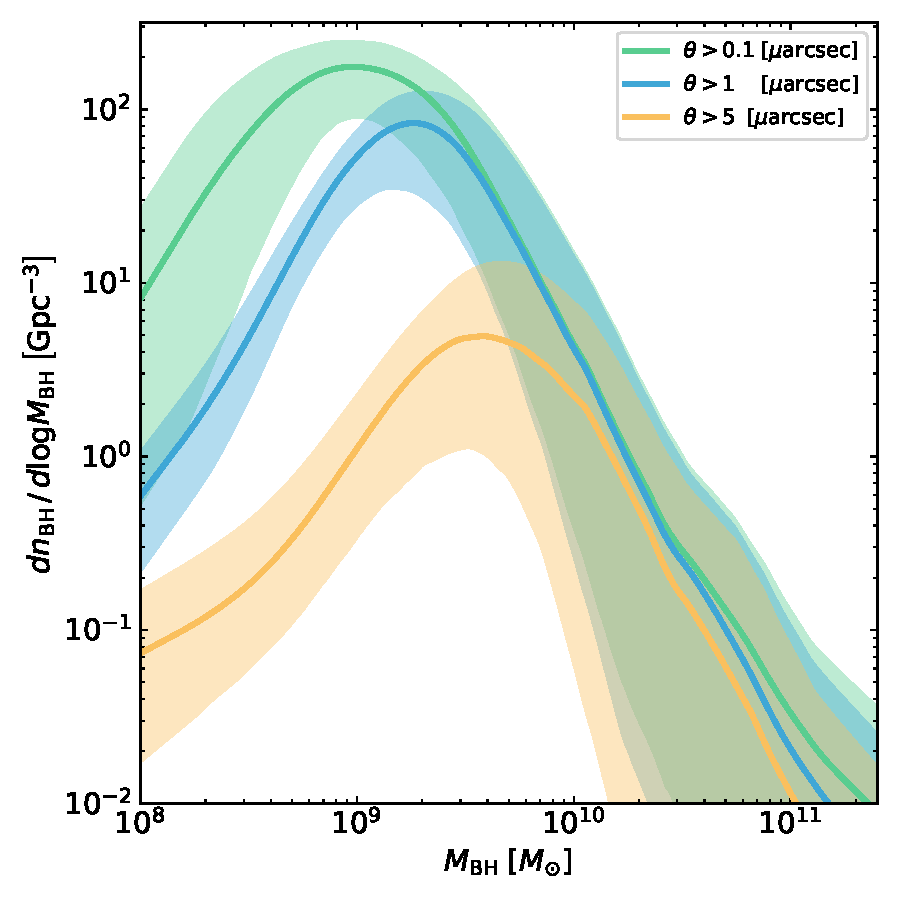
\includegraphics[width=0.48\textwidth]{Figs/mass_shad.pdf}
\begin{figure*}
    \centering
    \begin{subfigure}
        \centering
        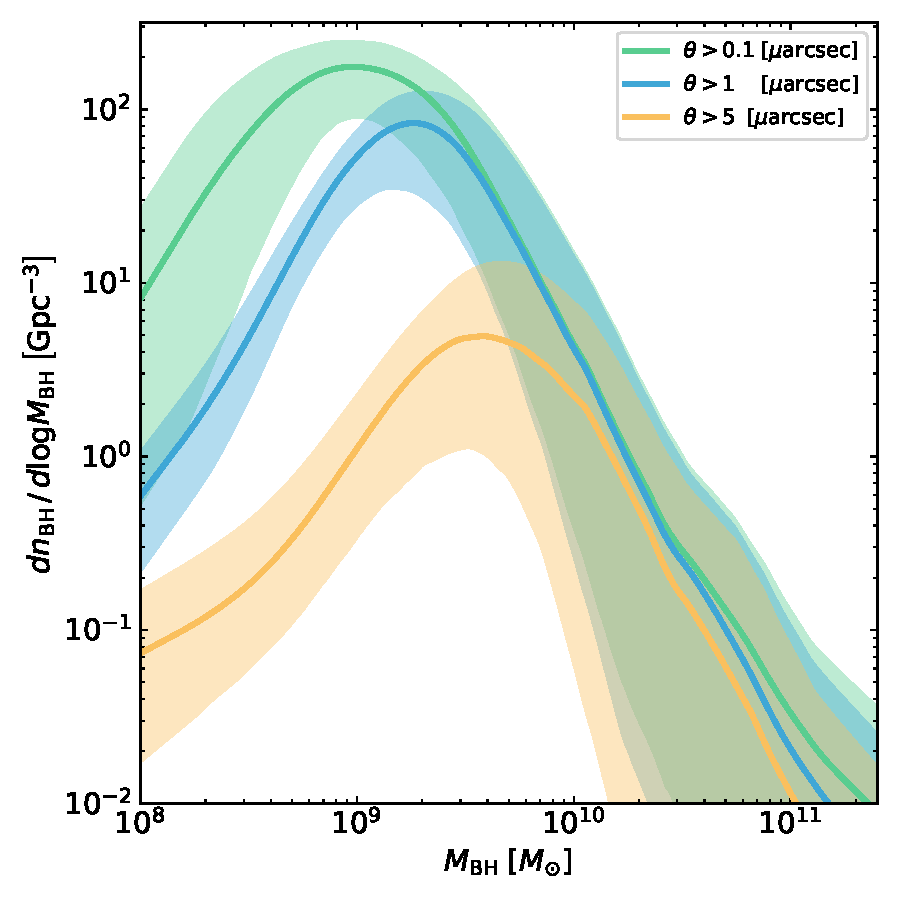
\includegraphics[width=0.48\linewidth]{Figs/mass_shad.pdf}
    \end{subfigure}
    ~
    \begin{subfigure}
        \centering
        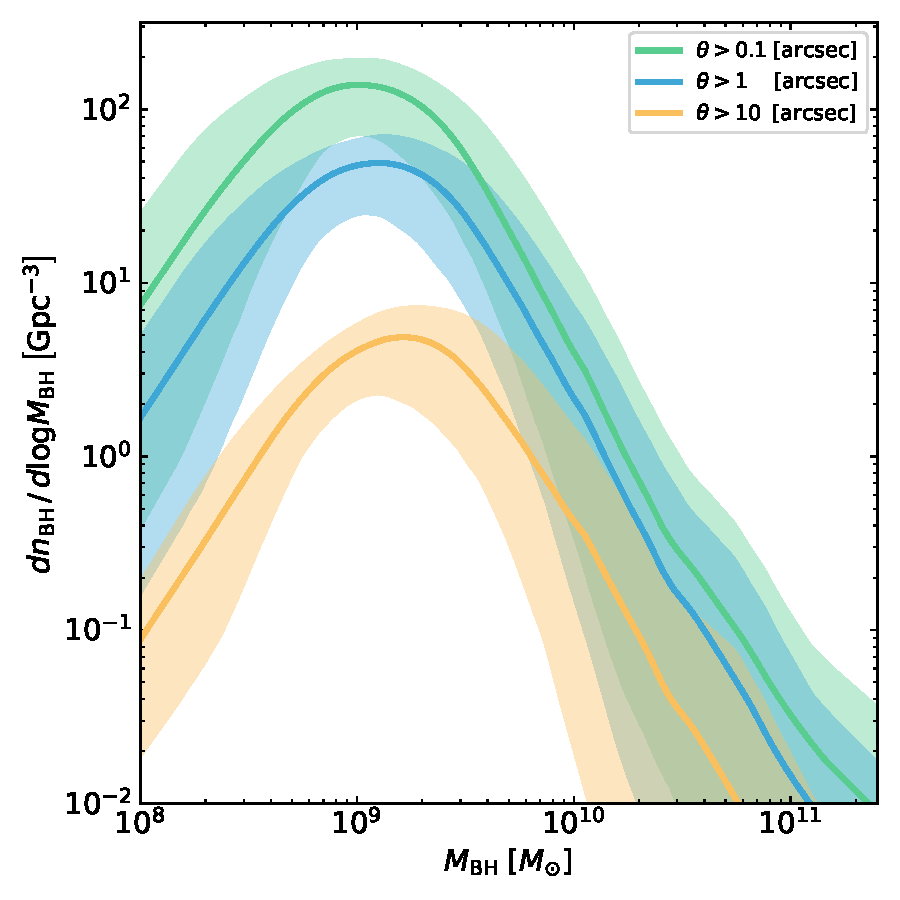
\includegraphics[width=0.48\linewidth]{Figs/mass_grav.pdf}
    \end{subfigure}
    \caption{BH mass function \label{fig:Mass_Funcion}}
\end{figure*}


\begin{figure*}
    \centering
    \begin{subfigure}
        \centering
        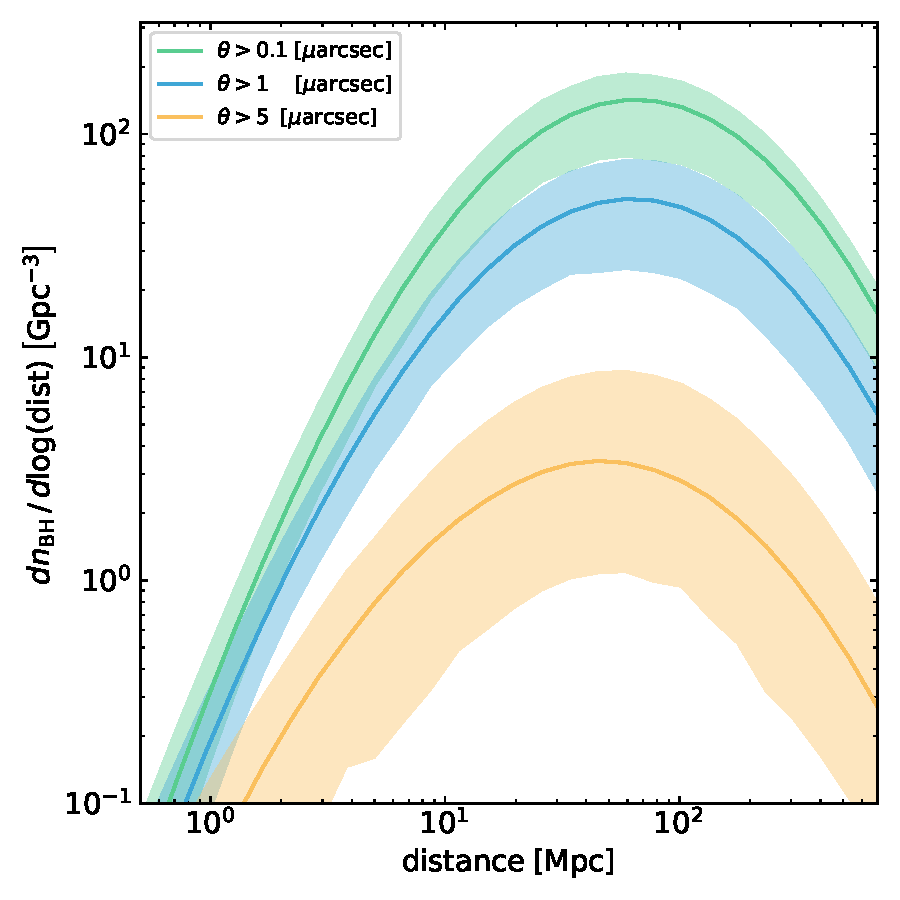
\includegraphics[width=0.48\linewidth]{Figs/dist_shad.pdf}
    \end{subfigure}
    ~
    \begin{subfigure}
        \centering
        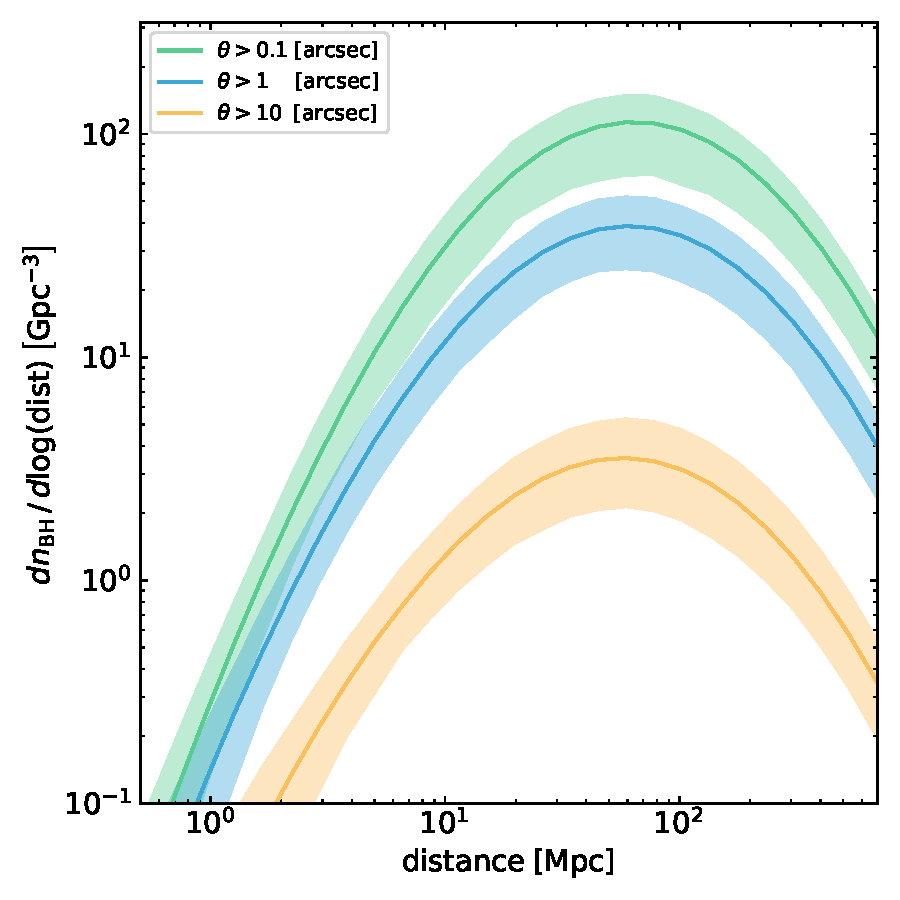
\includegraphics[width=0.48\linewidth]{Figs/dist_grav.pdf}
    \end{subfigure}
    \caption{BH distance function \label{fig:Dist_Function}}
\end{figure*}


\begin{figure*}
    \centering
    \begin{subfigure}
        \centering
        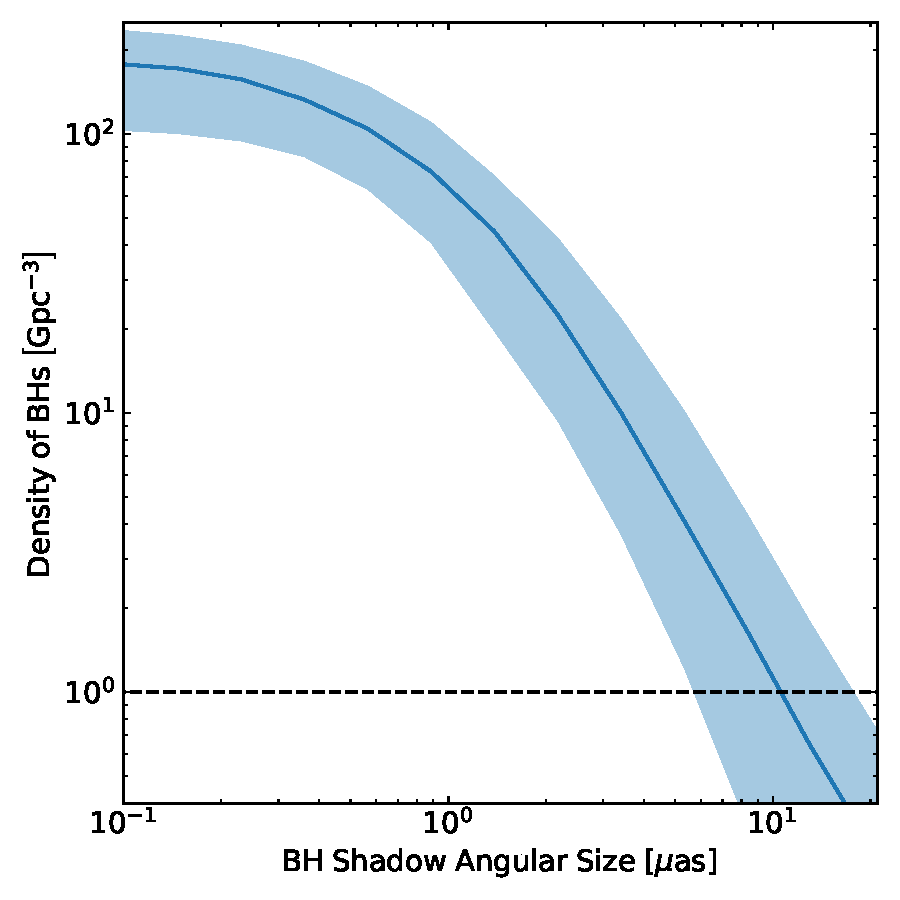
\includegraphics[width=0.48\linewidth]{Figs/tot_shad.pdf}
    \end{subfigure}
    ~
    \begin{subfigure}
        \centering
        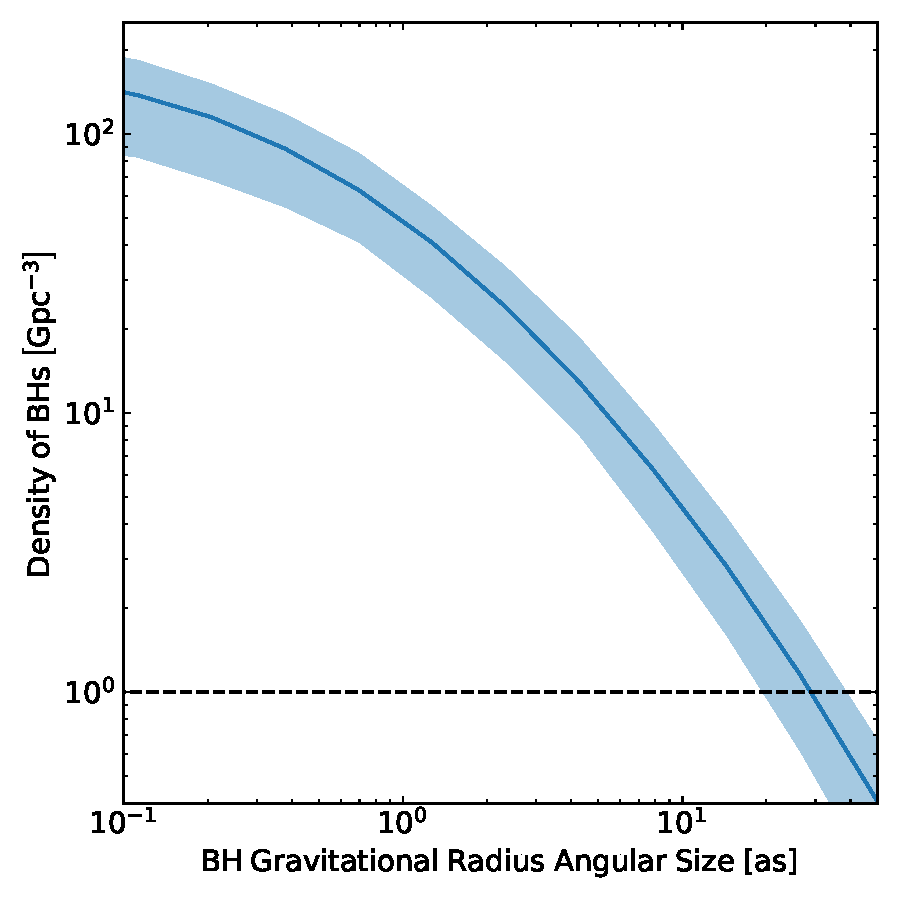
\includegraphics[width=0.48\linewidth]{Figs/tot_grav.pdf}
    \end{subfigure}
    \caption{Predicted number of BHs as a function of resolution \label{fig:Total_No.}}
\end{figure*}


\section{Method}
The SDSS provides us with measurements of quasars mass and position, while we are interested in determining the local abundance of BHs. To map the density of quasars into that of BH we make use 

\section{Results}




\section{Discussion}


\section*{Acknowledgements}



\bibliography{main}


\end{document}